%*****************************************
\chapter{Lab 03: Common Descriptive Measures}\label{ch:lab03}
%*****************************************
%\setcounter{figure}{10}
%\NoCaseChange{Homo Sapiens}

\section{Introduction}

One of the goals of descriptive statistics is to summarize and characterize the data so data scientists can determine its value and whether further research is needed. Often a simple measure like comparing the mean and median for a dataset can indicate a problem with outliers or skew. There are many statistics that are reported as descriptives and this lab both defines and demonstrates how those statistics are generated with \acs{PSPP}.\footnote{The information about calculated statistics in this lab is dependent on the datatypes discussed in Lab 1.}

\section{Discussion}

Each of the following sections describe one commonly-used statistical measure.

\subsection{Hinges}\label{lab03_hinges}

Occasionally, the phrase ``Tukey's Hinges'' appears in statistical literature. The two hinges for a dataset are the medians for the lower half and the upper half of the data, but those halves also include the dataset median. For the simple dataset above, the lower hinge is the median of $ 5 $, $ 7 $, $ 10 $, and $ 13 $, or $ 8.5 $. The upper hinge is the median of $ 13 $, $ 17 $, $ 19 $, and $ 23 $, or $ 18 $. Quartiles and hinges usually have about the same accuracy but quartiles are more commonly used.

\subsection{Inter-Quartile Range}\label{lab03_iqr}

Another measure that is occasionally used is the Inter-Quartile Range (\textit{IQR}); that is, the difference between \textit{Q1} and \textit{Q3}. This is used to produce a better range for an element in a dataset that includes extreme outliers.

\subsection{Kurtosis}\label{lab03_kurt}

One way to mathematically describe a normal distribution is to calculate the length of the tails of a bell curve, and that is called its \textit{excess kurtosis}. For a normal distribution the excess kurtosis is $ 0.00 $, a positive excess kurtosis would indicate longer tails while a negative excess kurtosis would indicate shorter tails. Intuitively, many people believe the excess kurtosis represents the ``peaked-ness'' of the curve since longer tails would tend to lead to a more peaked graph; however, excess kurtosis is a measure of the data outliers, which would be only present in the tails of the graph; so excess kurtosis is not directly indicative of the the ``sharpness'' of the peak. It is difficult to categorically state that some level of excess kurtosis is good or bad. In some cases, data that form a graph with longer tails are desired but in other cases they would be a problem.

Following are three examples of excess kurtosis. Notice that as the excess kurtosis increases the tails become longer. 

\begin{figure}[H]
  \begin{center}
    \fbox{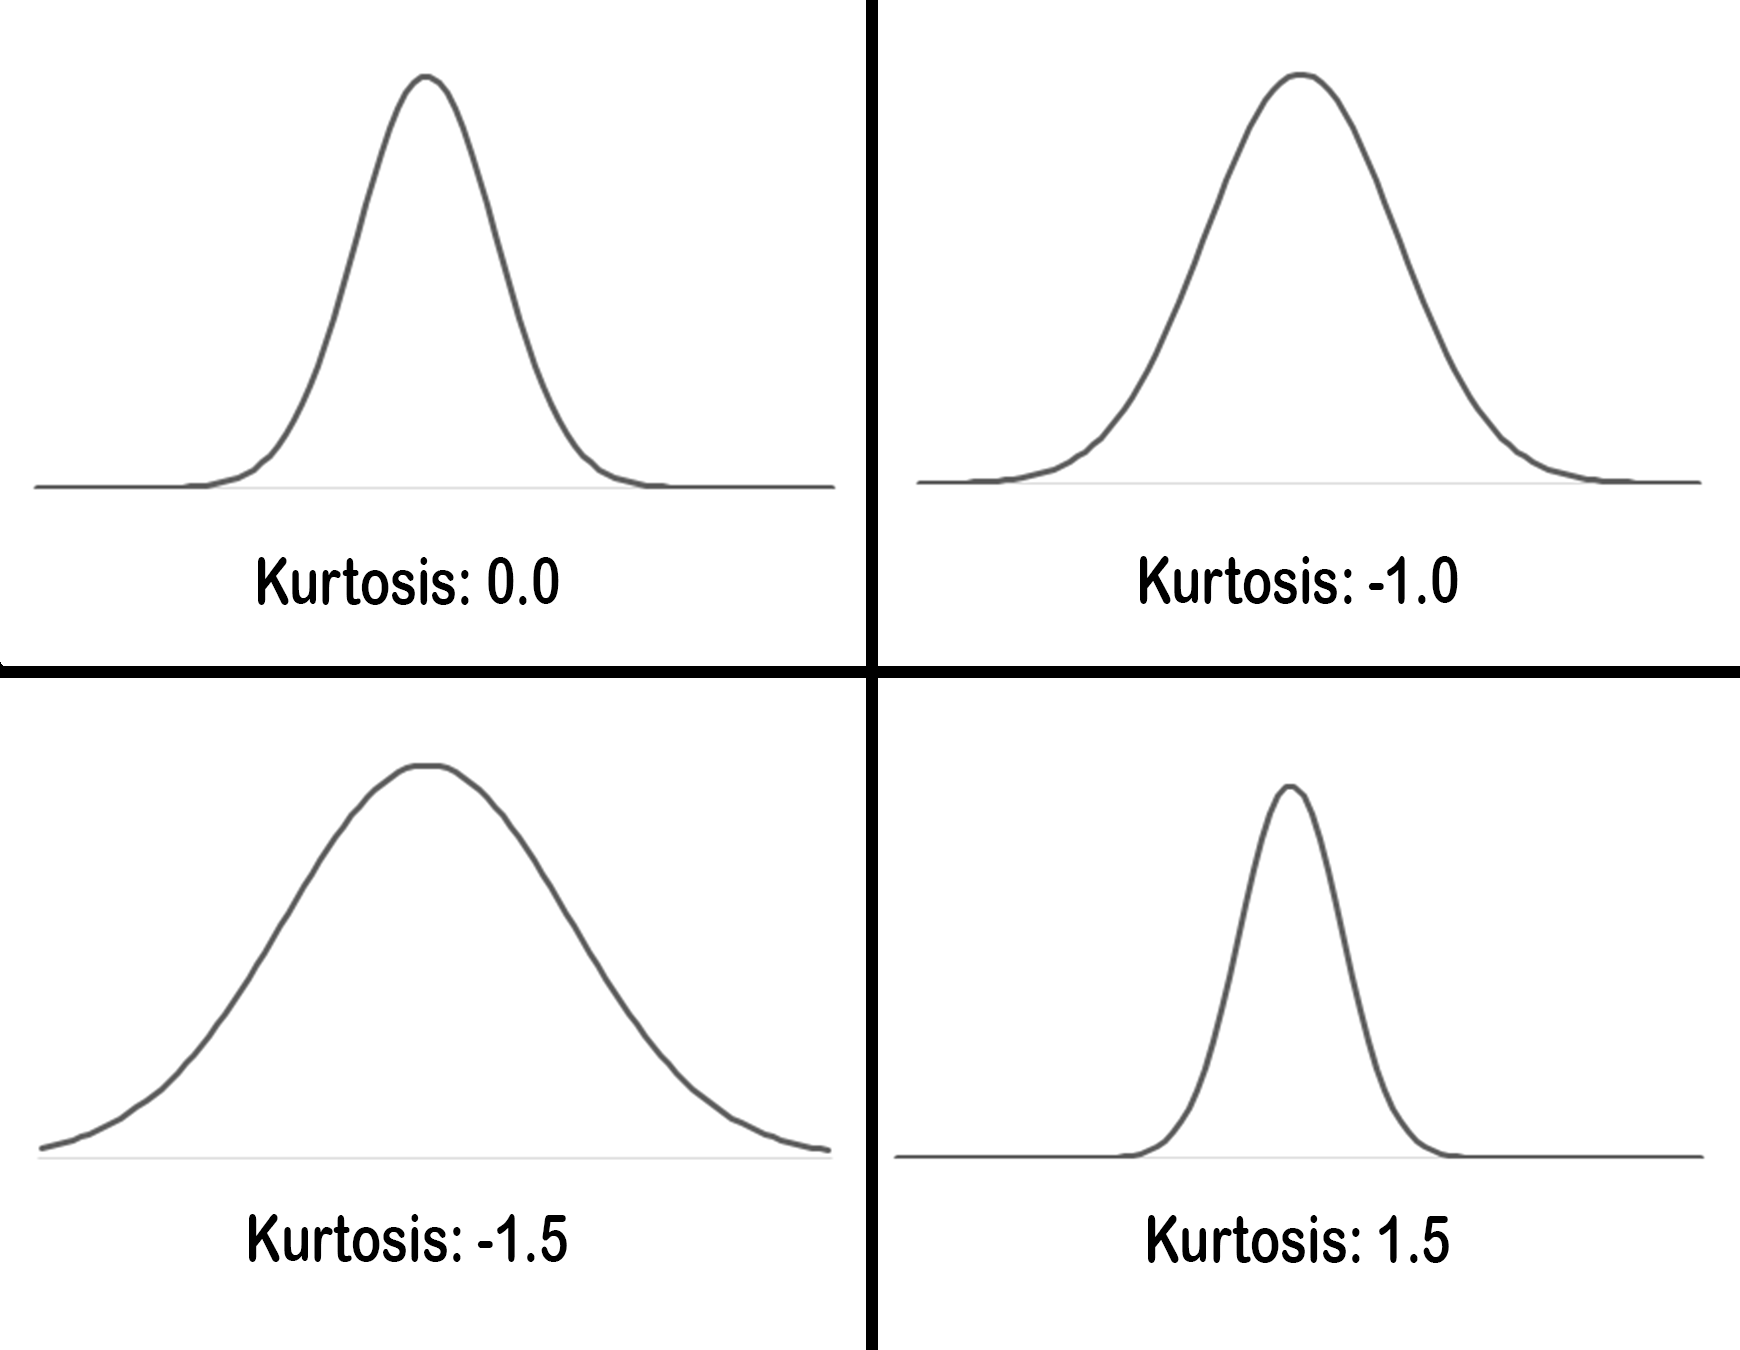
\includegraphics[width=\linewidth]{gfx/lab03_fig02}}
  \end{center}
  \caption{Kurtosis in a Normal Distribution}
  \label{lab03_fig02}  
\end{figure}

\subsection{Mean}\label{lab03_mean}

The mean is calculated by adding all of the data items together and then dividing that sum by the number of items, which is taught in elementary school as the \textit{average}. For example, given the dataset: $ 6, 8, 9 $, the total is $ 23 $ and that divided by $ 3 $ (the number of items) is $ 7.66 $; so the mean of $ 6, 8, 9 $ is $ 7.66 $.

If a dataset has outliers, or values that are unusually large or small, then the mean is often skewed such that it no longer represents the ``average'' value. As an example, the length (in miles) of the $ 141 $ longest rivers in North America ranges from $ 135 $ to $ 3710 $ and the mean of these values is $ 591.18 $ miles\footnote{These data are found in the \textit{rivers} dataset.}. Unfortunately, because the lengths of the top few rivers are disproportionately higher than the rest of the values in the dataset (their lengths are \textit{outliers}), the mean is skewed upward. One way compensate for outliers is to use a \textit{trimmed mean} (sometimes called a \textit{truncated mean}). A trimmed mean is calculated by removing a specified number of values from both the top and bottom of the dataset and then finding the mean of the remaining values. In the case of the rivers dataset, if $ 5\% $ of the values are trimmed from the data (or $ 2.5\% $ from both the top and bottom) then the remaining items create a ``trimmed'' mean of $ 518.79 $. Trimming the dataset effectively removes both upper and lower outliers and produces a much more reasonable central value for this dataset. In actual practice, a trimmed mean is not commonly used since it is difficult to know how much to trim from the dataset and the resulting mean may be just as skewed as if no values were trimmed; thus, when outliers are suspected, the best ``middle'' term to report is the median.

\subsection{Median}\label{lab03_median}

The median is found by listing all of the data items in numeric order and then mechanically finding the middle item. For example, using the dataset $ 6, 8, 9 $, the middle item (or median) is $ 8 $. If the dataset has an even number of items, then the median is calculated as the mean between the two middle items. For example, in the dataset $ 6, 8, 9, 13 $ the median is $ 8.5 $, which is the mean of $ 8 $ and $ 9 $, the two middle terms.

The median is very useful in cases where the dataset has outliers. As an example of using a median rather than a mean, consider the dataset $ 5, 6, 7, 8, 30 $. The mean is $ (5+6+7+8+30)/5 = 56/5 = 11.2 $. However, $ 11.2 $ is clearly much higher than most of the other numbers in that dataset since one outlier, $ 30 $, is significantly driving up the mean. A much better representation of the central term for this dataset would be $ 7 $, which is the median. To re-visit the river lengths introduced above, the median of the dataset is $ 425 $, which is much more representative of the ``middle'' length than using either the mean or the trimmed mean.

As another example, suppose a newspaper reporter wanted to find the ``average'' wage for a group of factory workers. The ten workers in that factory all have an annual salary of $ \$25,000 $; however, the supervisor has a salary of $ \$125,000 $. In the newspaper article, the supervisor is quoted as saying that the employees in his company have an average salary of $ \$34,090 $. That is correct if the mean of all those salaries is reported, but that number is clearly higher than any sort of reasonable ``average'' salary for workers in the factory due to the one outlier (the supervisor's salary). In this case, the median of $ \$25,000 $ would be much more representative of the ``average'' salary. The median is typically reported for salaries, home values, and other datasets where one or two outliers would significantly distort the reported ``middle'' value.

If the dataset contains no outliers and is normally distributed\footnote{The Normal Data Distribution, along with the terms skew and kurtosis, is covered in Lab 1.}, then the mean and median are the same; but if there are outliers then these two measures become separated, often by a large amount. Consider the rivers dataset mentioned in the \textit{Mean} section above. That dataset has a mean of $ 591.18 $ and a median of $ 425 $. This difference, $ 166.18 $, is about $ 28\% $ of the mean and is significant. The size of this difference would tell a researcher that there are outliers or other influences that are skewing the data.

\subsection{Minimum/Maximum}\label{lab03_min_max}

The minimum and maximum values of an element in a dataset are, as the name implies, the smallest and largest values. As an example, the dataset $ 6, 7, 8, 9, 10 $ has a minimum of $ 6 $ and a maximum of $ 10 $. The \textit{rivers} dataset has a minimum of  $ 135 $ and a maximum of $ 3710 $. 

\subsection{Mode}\label{lab03_mode}
The mode is used to describe the center of nominal or ordinal data and is nothing more than the value that is most often found in the dataset. For example, if a question asked respondents to select their zip code from a list of five local codes and ``$ 12345 $'' was selected more often than any other then that would be the mode for that item. Calculating the mode is no more difficult than counting the number of times the various values are found in the dataset and reporting the value found most frequently. 

As an example, the \textit{cars} dataset includes the following types of drive trains:

\rowcolors{1}{gray!25}{}
\begin{center}
  \begin{tabular}{lr}
    \hline 
    \textbf{Type} & \textbf{Frequency} \\ 
    \hline 
    $ 4 $WD & 2 \\ 
    Front & 43 \\ 
    Rear & 9 \\ 
    \hline 
  \end{tabular}
\end{center}

Since the most common type of drive train is ``Front'' that would be the mode for this data item.

It does not make much sense to calculate the mean or median for nominal or ordinal data since those are categories; however, reports frequently contain the mean for Likert-style questions (ordinal data) by equating each level of response to a number and then calculating the mean of those numbers. For example, imagine that a student housing survey asked respondents to select among ``Strongly Disagree, Disagree, Neutral, Agree, Strongly Agree'' for a statement like ``I like the food in the cafeteria.'' That is clearly ordinal data and while ``Agree'' is somehow better than ``Disagree'' it would be wrong to try to quantify that difference as ``one point better.'' Sometimes, though, researchers will assign a point value to those responses like ``Strongly Disagree'' is one point, ``Disagree'' is two points, and so forth. Then they will calculate the mean for the responses on a survey item and report something like ``The question about the food in the cafeteria had a mean of $ 3.24 $.'' It would be impossible to know what that means. Are students $ 0.24 $ units above ``Neutral'' on liking the cafeteria food? Thus, the mean or median should not be reported for nominal or ordinal data.

\subsection{N}\label{lab03_n}

One of the simplest of measures is nothing more than the number of items in a dataset. For example, the dataset $ 5, 7, 13, 22 $ contains $ 4 $ items. In statistics, the number of items in a dataset is usually represented by the letter \textit{N}, therefore, in the simple dataset in this paragraph, $ N = 4 $. 

\subsection{Quartiles}\label{lab03_quartiles}

A measure that is closely related to the median is the first and third quartile. The first quartile (\textit{Q1}) is the score that splits the lowest $ 25\% $ of the values from the rest and the third quartile (\textit{Q3}) splits the highest $ 25\% $ of the values from the rest. The second quartile (\textit{Q2}) is the same as the median and, normally, the term ``median'' is used rather than \textit{Q2}. For example, consider this dataset: 

\begin{center}
  $ 5, 7, 10, 13, 17, 19, 23 $
\end{center}

The median of this dataset is $ 13 $ because three values are smaller and three are larger. The first quartile is $ 7 $, which is the median for the lower half of the values (not including $ 13 $, the median of the dataset); or the score that splits the lowest $ 25 \% $ from the rest of the data. The third quartile is $ 19 $, which is the median for the upper half of the scores; or the score that splits the highest $ 25 \% $ from the rest of the data. 


\subsection{Range}\label{lab03_range}

The range of an element in a dataset is the maximum value minus the minimum value. As an example, the dataset $ 6, 7, 8, 9, 10 $ has a range of $ 10-6 $ or $ 4 $. The \textit{rivers} dataset has a range of $ 3575 $.

\subsection{Skew}\label{lab03_skew}

The second numerical measure of a normal distribution that is frequently reported is its \textit{skew}, which is a measure of the symmetry of the curve about the mean of the data. The normal distribution in Figure \ref{int:normal_dist_figure} has a skew of $ 0.00 $. A positive skew indicates that the tail on the right side is longer, which means that there are several data points on the far right side of the graph ``pulling'' the tail out that direction. A negative skew indicates that the tail on the left side of the graph is longer. Following are three examples of skew:

\begin{figure}[H]
  \begin{center}
    \fbox{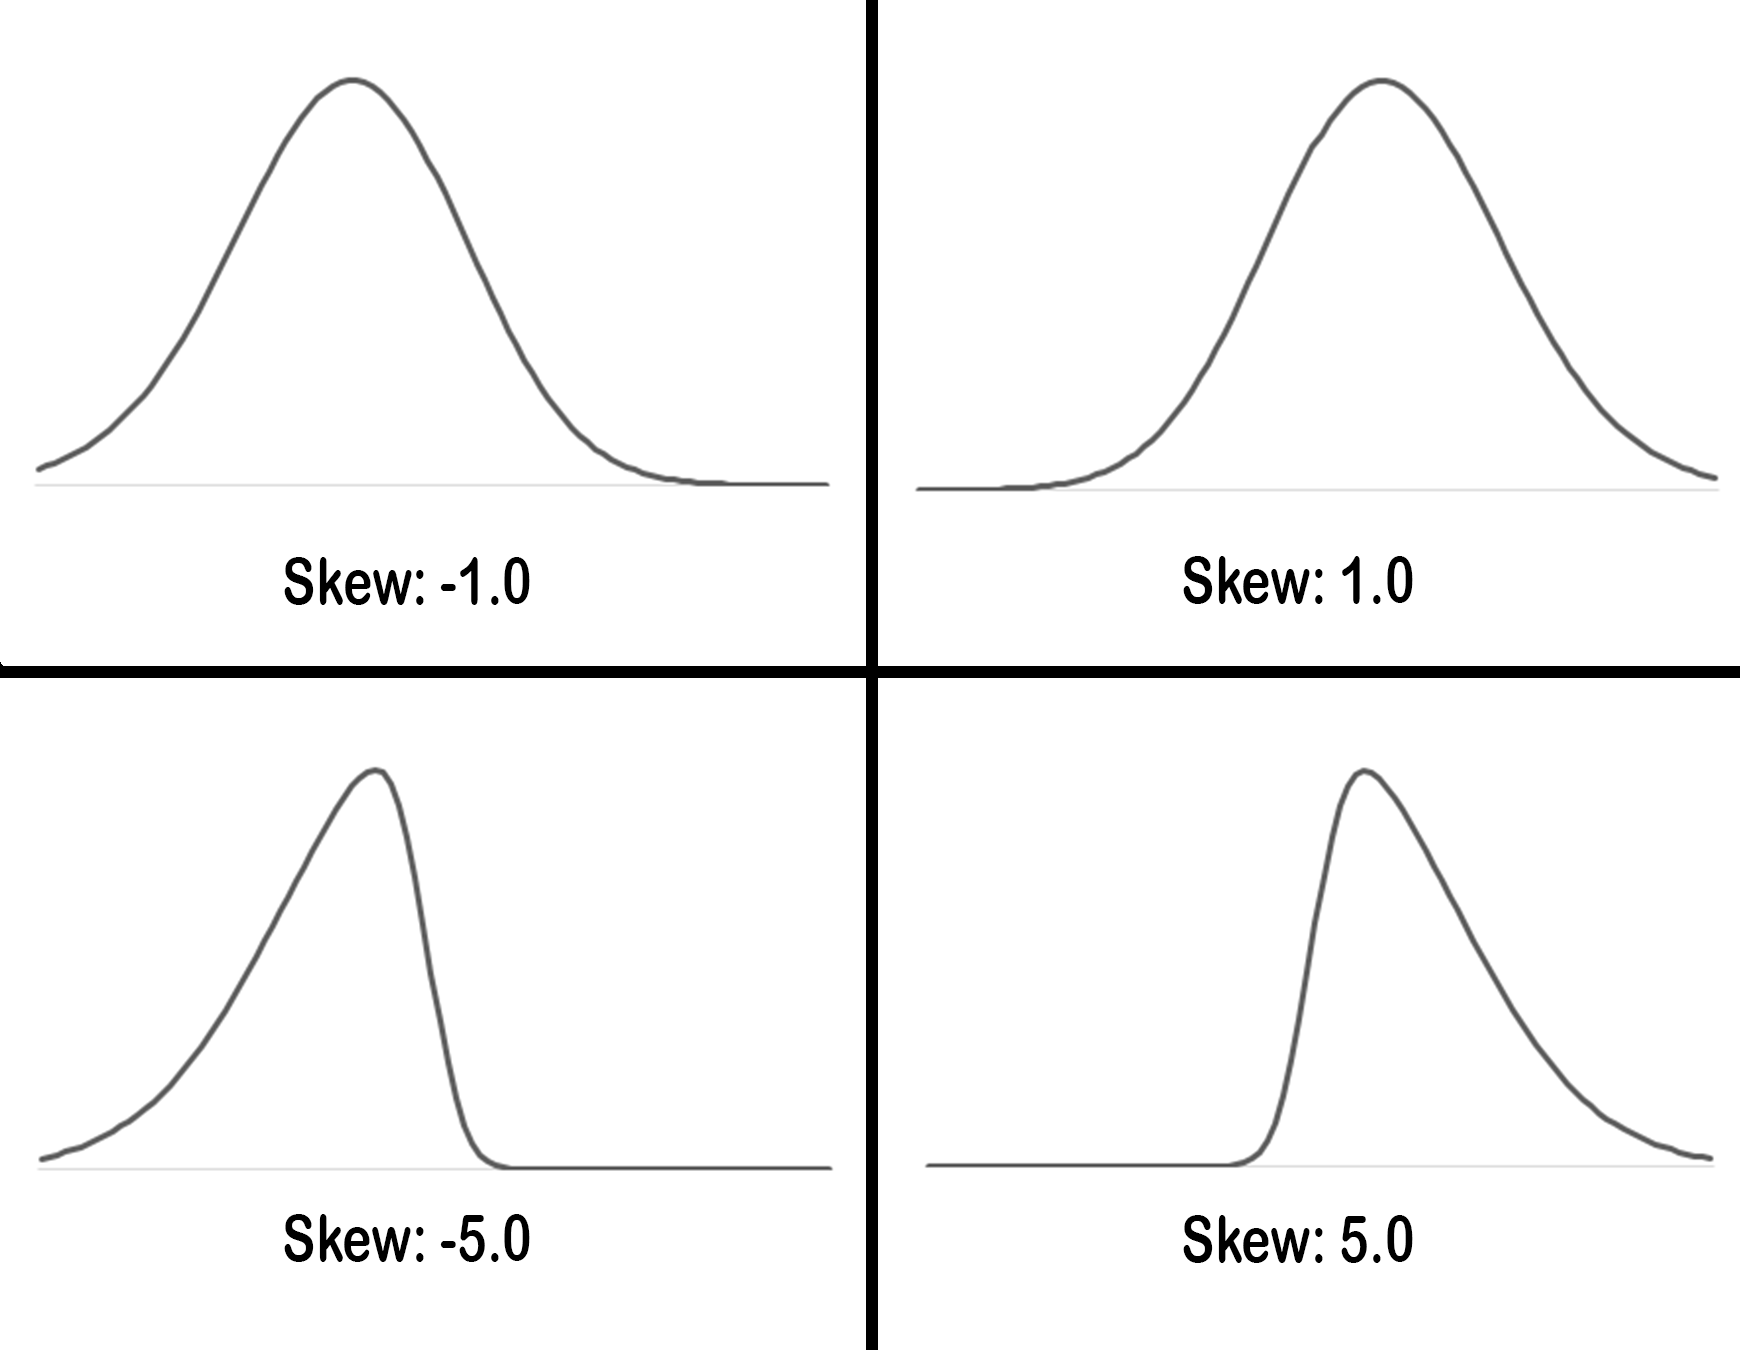
\includegraphics[width=\linewidth]{gfx/lab03_fig03}}
  \end{center}
  \caption{Skew in a Normal Distribution}
  \label{lab03_fig03}
\end{figure}

\subsection{Standard Deviation}\label{lab03_standard_deviation}

The standard deviation of a dataset is a number that indicates how much variation there is in the data; or how ``scattered'' the data are from the mean. In general, the larger the standard deviation then the more variation there is in the data. A dataset with a small standard deviation would create a sharply peaked normal distribution curve while a large standard deviation would create a flatter curve.\footnote{The concept of the normal distribution curve was presented in Lab 01.}

Once a standard deviation is calculated, then about $ 68.2 $\% of the samples will lie closer to the mean than that number. To put it another way, one standard deviation explains about $ 68.2 $\% of the variance from the mean. To show this concept graphically, consider the following graph of the scores on an examination:

\begin{figure}[H]
  \begin{center}
    \fbox{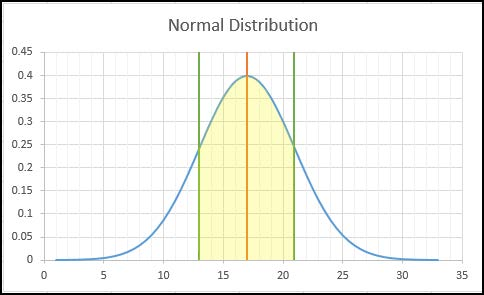
\includegraphics[width=\linewidth]{gfx/lab03_fig01}}
    \caption{Illustration Of Standard Deviation}
    \label{lab03_fig01}
  \end{center}
\end{figure}

The mean of this distribution is marked with a vertical line in the center of the bell curve. One standard deviation up and one standard deviation down are marked by two other vertical lines. The shaded area under the curve would include about $ 68.2 $\% of all scores for this dataset. In the same way, two standard deviations from the mean would include about $ 95.4 $\% of the data points; and three standard deviations would include more than $ 99.7 $\% of the data points (the second and third standard deviation are not indicated on the graph).

As one last example, imagine a class with $ 500 $ students where the professor administered an examination worth $ 100 $ points. If the mean score for that examination was $ 80 $ and the standard deviation was $ 5 $, then the professor would know that the scores were fairly tightly grouped ($ 341 $ scores of the $ 500 $ ($ 68.2 $\%) were between $ 75-85 $, within $ 5 $ points of the mean), and this would probably be good news for the professor. On the other hand, if the mean score was $ 60 $ and the standard deviation was $ 15 $, then the scores were ``all over the place' (more precisely, $ 341 $ scores of the $ 500 $ were between $ 45 $-$ 75 $), and that may mean that the professor would have to re-think how the lesson was taught or that the examination itself was flawed.

It is difficult to categorically state whether a specific standard deviation is good or bad; it is simply a measure of how concentrated the data are around the mean. For something like a manufacturing process where the required tolerance for the parts being produced is tight then the standard deviation for the weights of random samples pulled off of the line must be very small; that is, the parts must be as nearly identical as possible. However, in another context, the standard deviation may be quite large. Imagine measuring the time it takes a group of high school students to run $ 100 $ yards. Some would be very fast but others would be much slower and the standard deviation for that data would likely be large. 

\subsection{Standard Error}\label{lab03_standard_error}

If multiple samples are taken of a large population the mean of each of those samples will be slightly different. The ``standard error of the mean'' is the same as the standard deviation for a single sample. As an example, imagine that the following dataset are all of the test scores for $ 100 $ students who took the same departmental final examination last fall: 34, 44, 46, 46, 50, 52, 52, 53, 54, 54, 55, 56, 57, 58, 58, 58, 59, 60, 60, 62, 62, 62, 62, 64, 64, 64, 65, 65, 65, 66, 67, 68, 68, 68, 68, 69, 69, 69, 69, 70, 70, 70, 70, 70, 70, 71, 71, 71, 72, 72, 73, 73, 73, 73, 74, 75, 75, 75, 75, 75, 76, 77, 77, 77, 78, 78, 78, 78, 79, 79, 79, 79, 79, 79, 79, 80, 80, 80, 80, 81, 81, 82, 85, 86, 86, 86, 86, 86, 87, 87, 87, 90, 92, 93, 95, 95, 97, 100, 100, 100

Of course, with only $ 100 $ data points it would be very easy to calculate various statistics with the entire population, but that would not be possible if the sample were tens-of-thousands so a sample would be drawn at random from the entire population and it would be assumed that the sample would represent the entire population. Imagine that, at random, the following samples of ten were drawn from the population above:

\begin{table}[H]
  \sffamily
  \begin{center}
    \begin{tabular}{|l|r|r|}
      \hline 
      Sample & Sum & Mean \\ 
      \hline 
      $ 50, 56, 64, 72, 72, 75, 79, 80, 80, 93 $ & $ 721 $ & $ 72.1 $ \\ 
      \hline 
      $ 58, 69, 70, 75, 78, 79, 80, 81, 86, 95 $ & $ 771 $ & $ 77.1 $ \\ 
      \hline 
      $ 46, 58, 66, 70, 73, 75, 79, 85, 95, 100 $ & $ 747 $ & $ 74.7 $ \\ 
      \hline 
      $ 54, 60, 62, 66, 68, 70, 70, 71, 71, 73 $ & $ 665 $ & $ 66.5 $ \\ 
      \hline 
      $ 69, 72, 73, 76, 77, 77, 79, 79, 79, 81 $ & $ 762 $ & $ 76.2 $ \\ 
      \hline 
    \end{tabular} 
  \end{center}
\end{table}

The mean of the randomly-drawn sample should be the same as the mean for the entire population. However, it would be possible that the sample included only the high scores and the mean for that sample would be far different from the mean for a sample of low scores. The table above lists five different means depending on the samples drawn.

The actual mean for this dataset is $ 72.14 $. The standard error of the mean is $ 4.12 $ so the means of samples of ten values drawn at random would be expected to fall between $ 59.78 $ and $ 84.50 $, which is three standard errors below and above the mean.

The standard error is a useful way to estimate how accurately the mean of a sample reflects the mean of the entire population.

\subsection{Standard Error of the Kurtosis}\label{lab03_standard_error_of_the_kurt}

Kurtosis is defined earlier in this lab. Like the mean of a randomly-drawn sample would be expected to differ from the mean of the entire population (expressed as the Standard Error), the kurtosis of a randomly-drawn sample would be expected to differ from the kurtosis of the entire population. That expected difference would be expressed as the Standard Error of the Kurtosis.

\subsection{Standard Error of the Skew}\label{lab03_standard_error_of_the_skew}

Skew is defined earlier in this lab. Like the mean of a randomly-drawn sample would be expected to differ from the mean of the entire population (expressed as the Standard Error), the skew of a randomly-drawn sample would be expected to differ from the skew of the entire population. That expected difference would be expressed as the Standard Error of the Skew.

\subsection{Sum}\label{lab03_sum}

Another descriptor of a dataset that is occasionally reported is the sum, which is nothing more than the values of all of the items in an element added together. As an example, the dataset $ 6, 7, 8 $ has a sum of $ 21 $. The \textit{rivers} dataset has a sum of $ 83357 $. It should be rather obvious that the sum by itself does not offer much information without knowing the number of items in the dataset and the range of the values.

\subsection{Variance}\label{lab03_variance}

Statistically, the variance is a measure of how far a sample is spread out from the mean. A dataset with a wide variance would have values that are spread out ``all over the place'' while a dataset with a smaller variance would be more uniform. This is about the same definition that was used for Standard Deviation (page \pageref{lab03_standard_deviation}). In fact, there is a statistical relationship between variance and standard deviation: the standard deviation of a dataset is the square root of the variance. It is natural to wonder, then, which should be used. A standard deviation is measured with the same units as the dataset. So, for example, if some element of a dataset were measuring the height of all incoming students in inches then the standard deviation would also be in inches. Variance, on the other hand, is measured in square units so it is more difficult to compare the variance with the raw data. To be blunt, the variance has great utility in advanced statistics classes where students are considering theory but for most undergraduate classes where statistics are being used as a tool rather than the object of the study then the standard deviation is all that is needed.

\section{Procedure}

Labs Two through Six will generate most of the above measures so for this lab only a Frequency Table, as found in Lab Two, is used to generate a few simple statistics in this lab.

\subsection{Frequency Table with Statistics}

Start \acs{PSPP} and open the \textit{email} dataset, then:

\begin{enumerate}
  \item Click \textsc{\fbox{Analyze $ \rightarrow $ Descriptive Statistics $ \rightarrow $ Frequencies}}
  \item Click the word \textit{image} in the left column and then click the right-arrow button near the center of the window to move \textit{image} to the ``Variables'' box on the right side of the window. (Alternatively, double-click the word \textit{image} in the left column to move it to the ``Variables'' box.)
  \item Check \textit{Mean}, \textit{Minimum}, and \textit{Maximum} ``Statistics'' options in the lower-right box.
  \item Click \fbox{OK} to generate the frequency table.
\end{enumerate}

\begin{figure}[H]
  \begin{center}
    \fbox{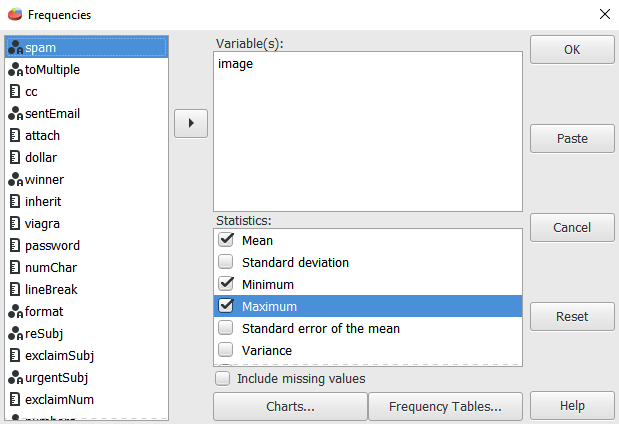
\includegraphics[width=\linewidth]{gfx/lab03_fig04}}
    \caption{Generating a Frequency Table With Statistics}
    \label{lab03_fig04}
  \end{center}
\end{figure}

\begin{figure}[H]
  \begin{center}
    \fbox{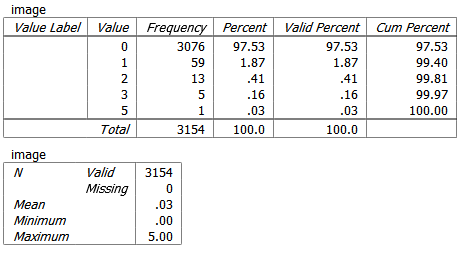
\includegraphics[width=\linewidth]{gfx/lab03_fig05}}
    \caption{Email Image Frequency Table With Statistics}
    \label{lab03_fig05}
  \end{center}
\end{figure}

Figure \ref{lab03_fig05} shows some simple statistics for the \textit{image} data element.\marginpar{Statics are only generated for Interval or Ratio data.}

\subsubsection{Activity 1: Frequency Table With Statistics} \label{lab03_act01}

Using the \textit{gifted} dataset, produce a frequency table for \textit{eduTV} (the number of hours children spend watching educational television programs each week). Include the \textit{mean}, \textit{minimum}, and \textit{maximum} values with the table.

\subsubsection{Activity 2: Frequency Table With Statistics} \label{lab03_act02}

Using the \textit{cafe} dataset, produce a frequency table for \textit{ptysize} (the size of the dining party). Include the \textit{mean}, \textit{minimum}, and \textit{maximum} values with the table.

\section{Deliverable}

Complete the following activities in this lab:

\rowcolors{1}{gray!25}{}
\begin{center}
  \begin{tabular}{lll}
    \hline 
    \textbf{Number} & \textbf{Name} & \textbf{Page} \\ 
    \hline 
    \ref{lab03_act01} & \nameref{lab03_act01} & \pageref{lab03_act01} \\ 
    \hline 
    \ref{lab03_act02} & \nameref{lab03_act02} & \pageref{lab03_act02} \\ 
    \hline 
  \end{tabular} 
\end{center}

Consolidate the responses for all activities into a single document and submit that document for grading.
